\documentclass[11pt]{article}

%opening
\usepackage{caption}
\usepackage{mcexam}
\usepackage{amsmath}
\usepackage{amsfonts}
\usepackage{graphicx}
\usepackage{enumerate}
\usepackage{tikz}
\usepackage{float}
\usepgflibrary{arrows}
\usepackage{todo}
\everymath{\displaystyle}
\pagestyle{empty}
\usepackage{lastpage} % this calculates the page number of the last page
\usepackage{fancyhdr}
\pagestyle{fancy}
\lhead{\textsf{Spring 2017}}
\chead{\textsf{Math 131 -- Midterm Exam 2A}}
\rhead{\textsf{Page \thepage\ of \pageref{LastPage}}}
\cfoot{}
\rfoot{\textsf{\thepage}}

\newcommand{\series}[3]{\displaystyle \sum_{{#1}={#2}}^{#3} }
\newcommand{\limit}[2]{\displaystyle \lim_{{#1} \rightarrow {#2}} }
\newcommand{\din}[2]{\displaystyle \int_{#1}^{#2}}
\newcommand{\Int}{\displaystyle \int}
\newcommand{\Q}{\ensuremath \mathbb{Q}}
\newcommand{\R}{\ensuremath \mathbb{R}}
\newcommand{\C}{\ensuremath \mathbb{C}}
\newcommand{\Z}{\ensuremath \mathbb{Z}}
\newcommand{\N}{\ensuremath \mathbb{N}}
\newcommand{\isom}{\ensuremath \cong}
\newcommand{\inv}{\ensuremath ^{-1}}
\newcommand{\ot}{\ensuremath \otimes}
\newcommand{\op}{\ensuremath \oplus}

\Course{Math 131}{Principles of Calculus}
\Instructor{Paul Gustafson}
\TestName{Exam 2A\hfill{\bfseries\Huge RED}}
\Date{}
%\Section{}


\begin{document}
\Head
\begin{instructions}
\item For questions which require a written answer, show all your work.  Full credit will be given only if the necessary work is shown justifying your answer.
\item Simplify your answers.
\item Calculators are allowed.
\item Should you have need for more space than is allocated to answer a question, use the back of the exam.
\item Please do not talk about the test with other students until exams are handed back.
\end{instructions}
\PointTable{2}
%\hrule width \linewidth height 2pt\vspace{2pt}%
%\hrule width \linewidth height 1pt\vspace{2pt}%
%\hrule width \linewidth height 1pt%
%\vspace{4mm}%
%\noindent {\bf For Instructor use only.}\\ \vspace{-.2in}%
%\begin{center}
%{\Large
%\begin{tabular}{|p{0.75in}|p{0.4in}|p{0.4in}|p{0.4in}|p{0.4in}|p{0.4in}|p{0.4in}|p{0.4in}|p{0.4in}|p{0.4in}|}
%\hline
%Question&MC&11&12&13&14&15&16&17&Total\\\hline
%Points&30&10&10&10&10&10&10&10&100\\\hline
%Earned&&&&&&&&&\\\hline
%\end{tabular}
%}
%\end{center}
\newpage

\vspace{.2in}

\noindent \emph{{\bf Part I: Multiple Choice (5 points each)} Mark the correct
answer on the bubble sheet.}
For questions 1-2, use the following graph of $f'(x)$:\\


\begin{minipage}{\linewidth}% to keep image and caption on one page
\centering
\makebox[\linewidth]{}
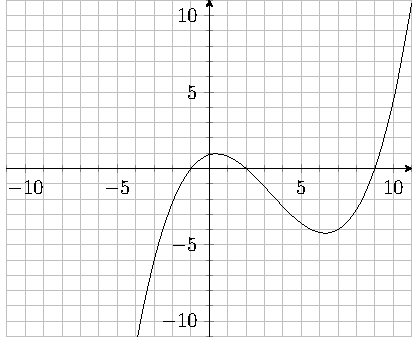
\includegraphics{exam2graph1.pdf}
\captionof{figure}{$f(x)$}\label{graph1exam1}%      only if needed  
\end{minipage}


\begin{questions}
\begin{multiplechoice}{5}
%8.5,8.6

\question According to the graph of $f'(x)$, the original function $f(x)$ has a local maximum at
\begin{answers}{3}
\ans $-1$
\ans $0.4$
\ans $2$
\ans $6.3$
\ans $9$
\end{answers}


\question According to the graph of $f'(x)$, the original function $f(x)$ is concave downward in which interval(s)?
\begin{answers}{3}
\ans $(-1,2) \cup (9, \infty)$
\ans $(-\infty, -1) \cup (2,9)$
\ans $(3, \infty)$
\ans $(0.4,6.3)$
\ans The original function is never concave down.
\end{answers}


\question Find the derivative of the function $f(x) = 5x^2 - 3x + 2$.
\begin{answers}{2}
\ans $10x + 2$
\ans $5x + 1$
\ans $ 5x -3$
\ans $10x +1$
\ans $10x - 3$
\end{answers}

\newpage

\question The graph of $g(x)$ is given below.\\

\begin{minipage}{\linewidth}% to keep image and caption on one page
\centering
\makebox[\linewidth]{}
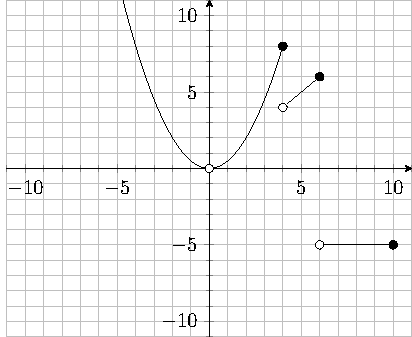
\includegraphics{exam2graph2.pdf}
\captionof{figure}{$g(x)$}\label{graph2exam1}%      only if needed  
\end{minipage}
\question According to the graph above, estimate the derivative of $g(x)$ at $x = 5$
\begin{answers}{2}
\ans $-\infty$
\ans -1
\ans 0
\ans 1
\ans The derivative does not exist at $x=5$.
\end{answers}

\question According to the graph above, estimate the derivative of $g(x)$ at $x = -2$
\begin{answers}{2}
\ans $-\infty$
\ans -1
\ans 0
\ans 1
\ans The derivative does not exist at $x= -2$.
\end{answers}


\question A vertical spring is released at time $t = 0$ seconds and begins to oscillate in a straight vertical line.
The height of its endpoint above the ground in meters is given by the function
$$h(t) = 5 - 0.1\cos(5t)$$
What is the velocity (in meters/second) of the spring's endpoint at time $t = 3$ ?
\begin{answers}{2}
\ans 0.28
\ans 0.13
\ans 0.33
\ans 5
\ans 0.46
\end{answers}

\newpage

\question Find the linear approximation to $(3x-5)^4$ at $x = 2$
\begin{answers}{2}
\ans $3x - 5$
\ans $12x - 23$
\ans $12x + 25$
\ans $-4x - 7$
\ans $-4x + 8$
\end{answers}


\question We are given an unknown function $f(x)$ such that $f'(3) = 0$, $f'(x) < 0$ for all $x > 3$, and $f'(x) > 0$ for all $x < 3$.
We can conclude that at $x = 2$, the function $f(x)$ has 
\begin{answers}{3}
\ans a local min.
\ans a local max.
\ans an inflection point.
\ans an undefined derivative.
\ans positive $y$-value.
\end{answers}

\question Calculate the equation of the tangent line to $y = 6 \sqrt{x} - 3$ at $x = 9$
\begin{answers}{2}
\ans $y = -2x + 5$
\ans $y = 3x + 25$
\ans $y = x + 6$
\ans $y = -2x -4$
\ans $y = 3x - 25$
\end{answers}


\question Find the derivative of the function $\displaystyle f(x) = \frac{3}{x^2 +1}$.
\begin{answers}{2}
\ans $ \displaystyle - \frac{6}{x^2 + 1}$
\ans $ \displaystyle  \frac{3 - 2x }{(x^2 + 1)^2}$
\ans $ \displaystyle  \frac{6}{(x^2 + 1)^2}$
\ans $ \displaystyle  - \frac{3}{2x}$
\ans $ \displaystyle  \frac{3}{2x}$
\end{answers}

\question Find the derivative of the function $\ln(\sec(x^2 e^x))$.
\begin{answers}{2}
\ans $(2x + x^2)e^x \tan(x^2 e^x)$
\ans $\tan(x^2 e^x)$
\ans $ \sec(x^2 e^x)\tan(x^2 e^x)$
\ans $(2x + x^2)e^x \sec(x^2 e^x)\tan(x^2 e^x)$
\ans $2x^2e^x \tan(x^2 e^x)$
\end{answers}

\end{multiplechoice}
\vspace{.2in}

\newpage

\noindent \emph{{\bf Part II: Free Response}{  Show all work}}
\question[14]  a.) (10 points) Using the \textbf{limit definition of derivative}, calculate the derivative of $f(x) = \sqrt{x + 3}$ at $x = 6$.
No points will be given for derivative rules or shortcuts.
\vspace{4.25in}

b.) (4 points) Calculate the equation of the tangent line to $f(x)$ at $x = 6$.


\newpage


\question[20] Calculate the derivative of the following functions. You may use the derivative rules to calculate
your answer. You do not need to simplify your answers.

a.) $\displaystyle f(x) = \frac{x^3 \ln(x)}{2x^2 -3}$
\vspace{3.25in}

b.) $\displaystyle f(x) = \cot(2^{(x^2 + 1)(x^4 - 1)})$
\vspace{3.25in}

\newpage

\question[15]   Use a linearization to estimate $\sqrt{16.3}$.  

\vspace{3.25in}


\question[15] Is the function
$$\begin{displaystyle}
f(x) = \begin{cases}
5x^2 - 8x, & x < 2 \\
3x^2 - 8, & x \ge 2
\end{cases}
\end{displaystyle}
$$
differentiable at $x = 2$? Why or why not?

\mbox{}
\end{questions}
\end{document}

*************************************************************************
*************************************************************************
